%!Tex Root = ../Tutorat6.tex
% ./Packete.tex
% ./Design.tex
% ./Deklarationen.tex
% ./Aufgabe1.tex
% ./Aufgabe3.tex
% ./Bonus.tex

\section{Task 2}

\setcounter{task}{1}

\begin{frame}[allowframebreaks]{Task 2}{Power Point Tracking Algorithm}
  \begin{requirementsnoinc}
    \begin{itemize}
      \item $I(U)=G \cdot 1 \mathrm{~A}-\left(\exp \left(\frac{U}{0.1 \mathrm{~V}}\right)-1\right) \cdot 0.01 \mathrm{~mA}$
      \item $P = I \cdot U$
    \end{itemize}
  \end{requirementsnoinc}
  \begin{solution}
    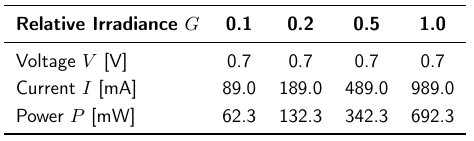
\includegraphics[width=\textwidth]{./figures/task2_sol1.png}
  \end{solution}
\end{frame}

\begin{frame}[allowframebreaks]{Task 2}{}
  \begin{tasknoinc}
    \begin{itemize}
      \item for $G=0.1$ and $G=1.0$
      \item $\triangle = 0.05V$
      \item iteration $k=1$, $V[0] = 0.7V$ and $V[1]=0.75V$
    \end{itemize}
  \end{tasknoinc}
  \begin{requirementsnoinc}
    \begin{itemize}
      \item $I(U)=G \cdot 1 \mathrm{~A}-\left(\exp \left(\frac{U}{0.1 \mathrm{~V}}\right)-1\right) \cdot 0.01 \mathrm{~mA}$
      \item $P = I \cdot U$
    \end{itemize}
    \centering
    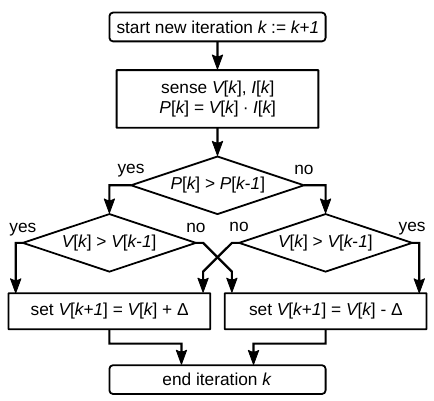
\includegraphics[height=0.3\textwidth]{./figures/task2_maximal_power_point_tracking.png}
  \end{requirementsnoinc}
  \begin{requirementsnoinc}
    \centering
    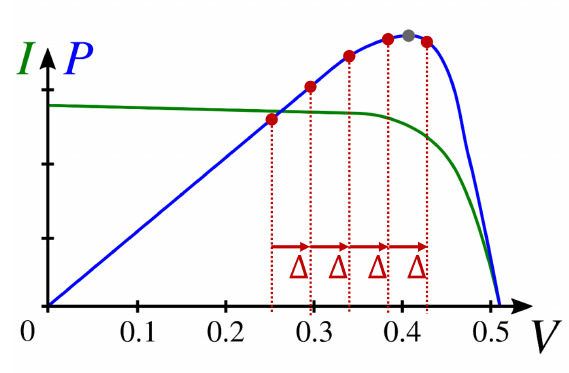
\includegraphics[width=0.5\textwidth]{./figures/task2_power_and_voltage.png}
  \end{requirementsnoinc}
  \begin{requirementsnoinc}
    \begin{itemize}
       \item $P(V)=V \cdot I(V)=V \cdot G-V \cdot\left(\exp \left(\frac{V}{0.1 \mathrm{~V}}\right)-1\right) \cdot 10^{-5}$
       \item the power $P$ extracted at a given operating point $V$, calculated as is a concave function of that $V$
       \item As the algorithm adjusts the operating point in discrete voltage steps $\triangle$, the maximum of the power $P[k]$ observed by the algorithm presents a lower bound of the actual maximum power point $P^{*}$.
        \begin{itemize}
          \item Only in the special case where the voltage of the maximum power point is a multiple of $\triangle$, it is matched exactly by the algorithm.
        \end{itemize}
    \end{itemize}
  \end{requirementsnoinc}
  \framebreak
  \begin{solutionnoinc}
     $G = 0.1$:
    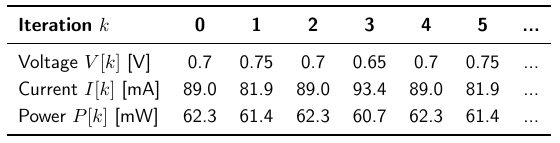
\includegraphics[width=\textwidth]{./figures/task2_sol2.png}
  \end{solutionnoinc}
  \begin{solution}
     $G = 1.0$:
    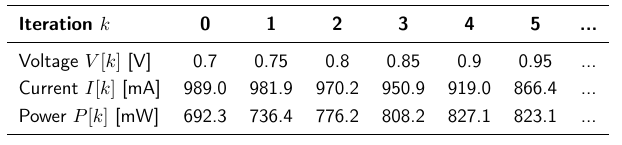
\includegraphics[width=\textwidth]{./figures/task2_sol3.png}
  \end{solution}
  \begin{tasknoinc}
    \centering
    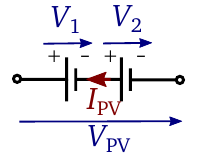
\includegraphics[width=0.3\textwidth]{./figures/task3_photovoltaic_panel.png}
  \end{tasknoinc}
  \begin{requirementsnoinc}
    \centering
    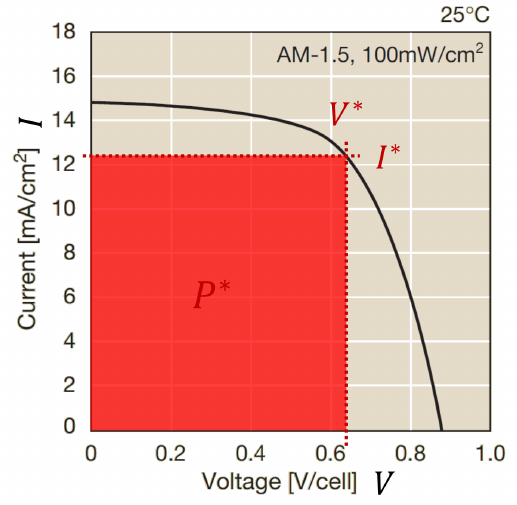
\includegraphics[width=0.4\textwidth]{./figures/task2_sweetspot.png}
  \end{requirementsnoinc}
  \begin{solutionnoinc}
    \begin{itemize}
      \item find the \alert{voltage} $V_1^*$ of the \alert{maximum power point} $P_1^*$ by numerically solving: $\displaystyle\frac{d}{d U_1} P_1\left(U_1\right)=\frac{d}{d U_1} U_1 \cdot I_1\left(U_1\right)$
      \item cell 1 with $G=1.0$: voltage at the maximum power point: $U_1^* \approx 0.919 \mathrm{~U}$ and the maximum power generated: $P_1^*=U_1^* \cdot I_1\left(U_1^*\right) \approx 829 \mathrm{~mW}$
      \item cell 2 with $G=0.1$: $U_2^*=0.712V$ and $P_2^*=62.4mW$
      \item  we determine an upper bound, i.e., a value which is larger than what can be generated by the partly shaded photovoltaic panel
      \item conditions: $U_{P V}=U_1+U_2 \quad$ and $\quad I_{P V}=I_1=I_2$
    \end{itemize}
  \end{solutionnoinc}
  \begin{solutionnoinc}
    \begin{itemize}
      \item $\begin{aligned}[t]
            & G_1-\left(\exp \left(\frac{U_1}{0.1}\right)-1\right) \cdot 10^{-5}=G_2-\left(\exp \left(\frac{U_2}{0.1}\right)-1\right) \cdot 10^{-5} \\
            & \Leftrightarrow\left(G_1-G_2\right) \cdot 10^5=\exp \left(\frac{U_1}{0.1}\right)-\exp \left(\frac{U_2}{0.1}\right) \\
            & \Leftrightarrow \exp \left(\frac{U_1}{0.1}\right)=\left(G_1-G_2\right) \cdot 10^5+\exp \left(\frac{U_2}{0.1}\right)
      \end{aligned}$
      \item $U_1=0.1 \cdot \log \left(\left(G_1-G_2\right) \cdot 10^5+\exp (0)\right) \approx 1.14 \mathrm{~V}$
      \item $P_{P V}=I_{P V} \cdot\left(U_1+U_2\right) \approx 114.1 \mathrm{~mW} = 0.1A \cdot\left(1.14V+0V\right) \approx 0.1141 \mathrm{~W} = 114.1 \mathrm{~mW}$
    \end{itemize}
  \end{solutionnoinc}
  \begin{solutionnoinc}
    \begin{itemize}
      \item The voltage $U_1 \approx 1.14 V$ at this operating point is already above $U_1^* \approx 0.919 V$ the maximum power point of cell 1. Therefore, an increase in $U_1$ (and $U_2$) results in a decrease in the output power for cell 1.
      \item safe upper bound: $P_{P V}^* \leq 176.5 \mathrm{~mW}=114.1 \mathrm{~mW}+62.4 \mathrm{~mW}$
      \item We note that this is significantly lower than $P_1^* \approx 829.0$ mW that can be generated with a single cell 1 at the same operating point. In addition, it is only slightly better than a situation, where both cells receive the low irradiance, namely $125 mW$
    \end{itemize}
  \end{solutionnoinc}
\end{frame}
